\section{Asure Blockchain}
From a technical point of view social security systems can be described as a number of rule-based (financial) transactions which are executed between a (usually) slightly changing total of different parties under the condition to maintain an equilibrium between deposited and withdrawn value over a period of time. Such a system can be implemented digitally by creating a blockchain-system, which supports smart contracts and cryptocurrencies.

Conventional social security systems currently generate up to hundreds million transactions per month, depending on the number of parties involved and the specific social security use-case. 

\begin{table}[H]
\centering
\begin{tabular}{lp{.2\textwidth}l}
  Monthly pension premiums & = 54.445 Mio\\
  Monthly pensions & = 25.646 Mio\\\hline
  Monthly pension transactions & = 80.091 Mio
\end{tabular}
\caption{\label{tab:table-name} For example the German statutory pension system: \cite{eckzahlen}}
\end{table}

In order to develop a blockchain system that can process these transactions, it is necessary to increase the achievable transaction throughput of the system and automatic batch processing within a transaction to reduce the number of total transactions to a minimum.

Both requirements can be addressed by the use of side-chains, as specified in the Plasma Framework. The Asure Blockchain functions as the scalable side-chain of the Asure Plasma implementation. It is the root-chain of the Asure Network and lays the foundation for optimal scalability regarding blockchain-based social security systems. 

Assets transferred from the Ethereum Blockchain to one of the Asure side-chains, are locked up in the Asure Plasma Contract on the Ethereum Blockchain until an exit transaction on the Ethereum Blockchain is executed. According to the Plasma MVP specifications, an equivalent of this value is created through the use of the operator design pattern (Proof-Of-Authority) on the Asure Blockchain and assigned to the user.

The available assets on the Asure Blockchain can then be used for transactions within the system. Consensus between all node providers within the Asure Blockchain is reached through a proof-of-stake consensus algorithm by using an adapted version of the Tendermint consensus engine. \cite{tendermint} Tendermint can handle transaction volume up to 10,000 transactions per second. With the help of zones and sharding concepts, this size can be increased by a factor of 1000. This would ensure the sustainable operation of social security on blockchain. \cite{tendermint_bench}

\begin{figure}[H]
    \centering
    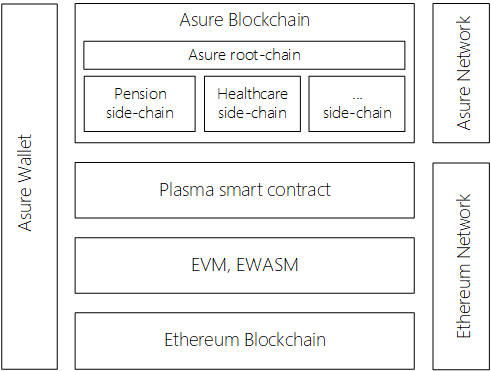
\includegraphics[width=4.0in]{img/architecture.png}
    \caption{Asure architecture}
    \label{fig:asure_architecture}
\end{figure}

The Asure Blockchain has several fundamentals. 

\subsection{Security}
The Asure Blockchain includes several features that protect it against such attacks as unauthorized spending, double spending, forging assets, and tampering with the blockchain. 

Each block added to the blockchain, starting with the block containing a particular transaction, is referred to as a confirmation of that transaction. Ideally, recipients and senders receiving payments should wait until at least one confirmation has been distributed across the network before assuming that the payment has been made. The more confirmations the recipient waits, the more difficult it is for an attacker to successfully reverse the transaction in a blockchain unless the attacker controls more than half of the total network performance, in which case it is called a 51\% attack. This construction is not designed to prevent 51\% of attacks, but rather to encourage block propagation. 

\subsection{Consensus algorithm}
There are different versions for proof algorithms. Proof-of-work is highly criticized because of enormous power consumption.\cite{hackernoon} Long-term acceptance and community movement is moving towards proof-of-stake where validators create the blocks and are rewarded for doing the correct job. The Asure blockchain will use a Proof-of-Stake (PoS) consensus algorithm. It will use in the first MVP implementation the Tendermint consensus engine.\cite{tendermint}

\subsection{Privacy with (ZK-SNARKS and ZK-STARK)}
Among other things, the Asure Blockchain takes into account privacy aspects that have an enormous relevance in relation to social security.

ZK-SNARKS (Zero-Knowledge Succinct Non-interactive Argument of Knowledge) offers the possibility to carry out anonymous transactions. The ZK-SNARKS are not resistant to Quantum Computing. ZK-STARK (Zero-Knowledge Scalable Transparent Argument of Knowledge) is the latest innovation aimed to achieve privacy on the blockchain with the use of fast, scalable computations and is resistant to Quantum Computing. \cite{iacr}

Since Ethereum is also researching in Layer 1 in this area, it will be possible for social security transactions to remain anonymous for those insured. \cite{ethereum_zksnarks}

The state of Zero-Knowledge technologies is not yet entirely practicable, but this will change in the future.

\subsection{EVM, WASM, eWASM, *WASM}
EVM provides a turing-complete computation so that Ethereum can run a general program, also known as a smart contract. Plasma EVM is a new version of Plasma that can execute EVM in plasma chain, and its clients can be based on current Ethereum clients (go-ethereum, py-evm, parity). We propose state-enforceable Plasma construction to guarantee only valid state submitted to root-chain, providing a way to enter and exit account storage between two chains because each chain has identical architecture. Another benefit is that Ethereum development tools can also be used in plasma chain.

eWASM is just an Ethereum "flavored" subset of Web Assembly, which is binary instruction format. eWASM  relies on instructions that are very close to real-world CPU. The performance improvements are significant and seem more secure. WebAssembly is backed by Mozilla, Google, Apple, and Microsoft, the community is also active, it's gonna be a widely used web standard.  

The Ethereum Blockchain processes about 15 transactions per second (TPS), which is not sufficient for the implementation of a social security system. The improvements to Ethereum (also called Layer 1), which are currently in progress, should significantly increase the number of TPS. Among the improvements are a Proof-of-Stake (PoS) based consensus algorithm, sharding, and by the introduction of eWASM - a WebAssembly based virtual machine.

\subsection{Further technologies}
Parity Substrate is a high-level framework for creating cryptocurrencies and other decentralized systems using the latest research in blockchain technology. 

Cosmos-SDK is a blockchain framework to allow developers to easily create custom interoperable blockchain applications within the Cosmos Network without having to recreate common blockchain functionality, thus removing the complexity of building a Tendermint ABCI application. We envision the SDK as the npm-like framework to build secure blockchain applications on top of Tendermint.

LotionJS aims to make writing new blockchains fast. It builds on top of Tendermint using the ABCI protocol. Lotion lets you write secure, scalable applications that can easily interoperate with other blockchains on the Cosmos Network.

